% Figure 1 (redesign): audit overview. Standalone TikZ; compile with pdflatex.
% Designed at the elsarticle preprint text width (~13.7 cm); fonts are 7-8.5 pt sans.
\documentclass[tikz,border=1pt]{standalone}
\usepackage[T1]{fontenc}
\usepackage[scaled=0.92]{helvet}
\renewcommand{\familydefault}{\sfdefault}
\usepackage{sansmath}
\sansmath
\usetikzlibrary{arrows.meta,positioning,calc}

% ---- palette (blue / orange validated for CVD separation on white) ----
\definecolor{ink}{HTML}{0B0B0B}
\definecolor{ink2}{HTML}{52514E}
\definecolor{muted}{HTML}{898781}
\definecolor{hair}{HTML}{C3C2B7}
\definecolor{grid}{HTML}{E1E0D9}
\definecolor{wash}{HTML}{F5F4F0}
\definecolor{refit}{HTML}{2A78D6}     % predictor change
\definecolor{refitwash}{HTML}{EAF2FC}
\definecolor{hist}{HTML}{EB6834}      % history change
\definecolor{histwash}{HTML}{FDEFE8}

\tikzset{
  >={Stealth[length=4pt,width=3.4pt]},
  every node/.style={font=\fontsize{7.5}{9}\selectfont, text=ink},
  box/.style={draw=hair, line width=0.6pt, rounded corners=2pt, fill=white,
              minimum height=0.95cm, align=center, inner sep=2.5pt},
  flow/.style={->, draw=ink2, line width=0.6pt},
  badge/.style={circle, fill=ink, text=white, inner sep=0pt, minimum size=0.34cm,
                font=\fontsize{6.8}{6.8}\selectfont\bfseries},
  panel/.style={font=\fontsize{8.5}{10}\selectfont\bfseries, anchor=base west},
  sub/.style={font=\fontsize{7}{8.4}\selectfont, text=ink2, anchor=base west},
  note/.style={font=\fontsize{6.8}{8.2}\selectfont, text=ink2, align=left},
  chip/.style={rounded corners=2pt, line width=0.6pt, align=left, inner sep=3.2pt, minimum height=1.20cm,
               anchor=north west, font=\fontsize{7}{8.6}\selectfont},
  % an image frame with a two-link arm: #1 shoulder angle, #2 elbow angle, #3 frame colour, #4 size
  pics/obs/.style args={#1/#2/#3/#4}{code={
     \draw[#3, line width=0.6pt, fill=white, rounded corners=1pt] (-#4,-#4) rectangle (#4,#4);
     \draw[ink2, line width=0.8pt, line cap=round, line join=round]
          (-0.35*#4,-0.30*#4) -- ++(#1:0.62*#4) -- ++(#2:0.50*#4);
     \fill[ink2] (-0.35*#4,-0.30*#4) circle (0.10*#4);
  }},
}

\begin{document}
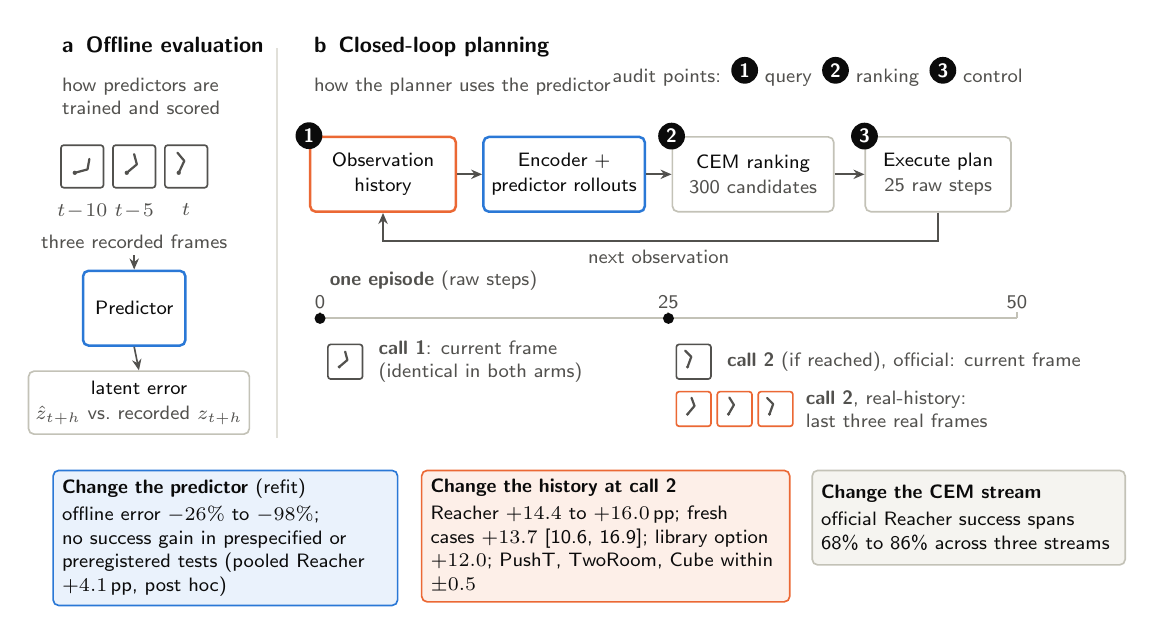
\begin{tikzpicture}
\hyphenpenalty=10000 \exhyphenpenalty=10000

% ================= (a) Offline evaluation =================
\node[panel] at (0,5.00) {a\enspace Offline evaluation};
\node[sub, align=left, anchor=north west] at (0,4.80) {how predictors are\\trained and scored};

% three recorded frames (arm moves between frames, so velocity is visible)
\foreach \i/\a/\b/\lab in {0/15/80/t\!-\!10, 1/40/105/t\!-\!5, 2/65/130/t}{
  \pic at (0.38+0.66*\i,3.55) {obs={\a/\b/ink2/0.27}};
  \node[note, anchor=north] at (0.38+0.66*\i,3.20) {$\lab$};
}
\node[note, anchor=north] at (1.04,2.80) {three recorded frames};

\node[box, draw=refit, line width=0.9pt, minimum width=1.30cm] (predA) at (1.04,1.75) {Predictor};
\draw[flow] (1.04,2.42) -- (predA.north);
\node[box, minimum width=1.9cm, minimum height=0.80cm] (errA) at (1.10,0.55)
      {latent error\\{\color{ink2}$\hat z_{t+h}$ vs.\ recorded $z_{t+h}$}};
\draw[flow] (predA.south) -- (errA.north);

% ================= (b) Closed-loop planning =================
\def\bx{3.20}
\node[panel] at (\bx,5.00) {b\enspace Closed-loop planning};
\node[sub, anchor=north west] at (\bx,4.80) {how the planner uses the predictor};
\node[note, anchor=base east] at (\bx+9.25,4.62) {audit points:\enspace\tikz[baseline=-0.6ex]\node[badge]{1}; query\enspace\tikz[baseline=-0.6ex]\node[badge]{2}; ranking\enspace\tikz[baseline=-0.6ex]\node[badge]{3}; control};

\node[box, draw=hist, line width=0.9pt, minimum width=1.85cm] (hist) at (\bx+1.00,3.45) {Observation\\history};
\node[box, draw=refit, line width=0.9pt, minimum width=2.05cm] (pred) at (\bx+3.30,3.45) {Encoder +\\predictor rollouts};
\node[box, minimum width=2.05cm] (cem)  at (\bx+5.70,3.45) {CEM ranking\\{\color{ink2}300 candidates}};
\node[box, minimum width=1.85cm] (exe)  at (\bx+8.05,3.45) {Execute plan\\{\color{ink2}25 raw steps}};

\draw[flow] (hist) -- (pred);
\draw[flow] (pred) -- (cem);
\draw[flow] (cem)  -- (exe);
\draw[flow] (exe.south) -- ++(0,-0.36) -| (hist.south);
\node[note, anchor=north] at (\bx+4.50,2.97-0.36) {next observation};

% where the audit measures (badge sits on the node corner)
\node[badge] at (hist.north west) {1};
\node[badge] at (cem.north west)  {2};
\node[badge] at (exe.north west)  {3};

% ---- one episode: at most one replanning call ----
\def\ty{1.62}
\def\tx{\bx+0.20}
\def\tw{8.85}
\node[note, anchor=base west] at (\tx,\ty+0.42) {\textbf{one episode} (raw steps)};
\draw[hair, line width=0.7pt] (\tx,\ty) -- (\tx+\tw,\ty);
\foreach \s/\lab in {0/0, 0.5/25, 1/50}{
  \draw[hair, line width=0.7pt] ($(\tx,\ty)+(\s*\tw,0)$) -- ++(0,0.08);
  \node[note, anchor=base] at ($(\tx,\ty)+(\s*\tw,0.13)$) {\lab};
}


% call 1 (identical in both arms)
\fill[ink] (\tx,\ty) circle (0.07);
\pic at ($(\tx,\ty)+(0.32,-0.55)$) {obs={40/105/ink2/0.22}};
\node[note, anchor=west] at ($(\tx,\ty)+(0.62,-0.55)$) {\textbf{call 1}: current frame\\(identical in both arms)};

% call 2: official vs real-history replanning
\coordinate (c2) at ($(\tx,\ty)+(0.5*\tw,0)$);
\fill[ink] (c2) circle (0.07);
\pic at ($(c2)+(0.32,-0.55)$) {obs={70/135/ink2/0.22}};
\node[note, anchor=west] at ($(c2)+(0.62,-0.55)$) {\textbf{call 2} (if reached), official: current frame};
\foreach \i/\a/\b in {0/50/110, 1/60/122, 2/70/135}{
  \pic at ($(c2)+(0.32+0.52*\i,-1.15)$) {obs={\a/\b/hist/0.22}};
}
\node[note, anchor=west] at ($(c2)+(1.62,-1.15)$) {\textbf{call 2}, real-history:\\last three real frames};

\draw[grid, line width=0.6pt] (2.85,5.05) -- (2.85,0.10);

% ================= result strip =================
\def\ry{-0.30}
\node[chip, draw=refit, fill=refitwash, text width=4.15cm] at (0,\ry)
  {\textbf{Change the predictor} (refit)\\[1pt]
   offline error $-26\%$ to $-98\%$; no success gain in prespecified or preregistered tests (pooled Reacher $+4.1$\,pp, post hoc)};
\node[chip, draw=hist, fill=histwash, text width=4.45cm] at (4.68,\ry)
  {\textbf{Change the history at call 2}\\[1pt]
   Reacher $+14.4$ to $+16.0$\,pp; fresh cases $+13.7$ [10.6, 16.9]; library option $+12.0$; PushT, TwoRoom, Cube within $\pm0.5$};
\node[chip, draw=hair, fill=wash, text width=3.75cm] at (9.64,\ry)
  {\textbf{Change the CEM stream}\\[1pt]
   official Reacher success spans 68\% to 86\% across three streams};

\end{tikzpicture}
\end{document}
